\section{Artificial Neural Networks}
\label{sec:rul_ann}

Although Artificial Neural Networks (\glspl{ann}) are widely know nowadays in this section we will briefly introduce the basic concepts behind them to provide the reader a better understanding of the tools used in this work. We will follow the notation and conventions used in \cite{Engelbrecht2007}

Artificial Neural Networks (\glspl{ann}) are systems vaguely inspired by the biological Neural Networks in the brain. Neurons are the building blocks of any type of \gls{ann}. The Artificial Neuron \gls{an}, or neuron, implements a nonlinear mapping from $\mathbb{R}^{n}$ to $\left[a,b\right]$ where $n$ is the number of inputs the \gls{an} receives and $a$ and $b$ depend on the chosen activation function. Usual combinations for $a$ and $b$ are $\left[0,1\right]$ or $\left[-1,1\right]$

\begin{equation}
f_{AN} : \mathbb{R}^n \rightarrow \left[a,b\right]
\label{eq:an_def}
\end{equation}

An \gls{an} receives a vector of $n$ input signals, $\mathbf{z} = (z_1, z_2, \cdots , z_n)$, either from the environment or from other \glspl{an}. The \gls{an} computes the net input signal, and uses an activation function $f_{AN}$ to compute the output signal, $o$, given the net input. The strength of the output signal is further influenced by a bias value $\theta$. Figure \ref{fig:an_1} presents an illustration of an \gls{an}.

\begin{figure}[h]
    \centering
    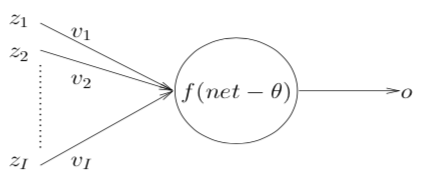
\includegraphics[width = 50mm, height = 25mm]{img/artificial_neuron.png}
    \caption{An Artificial Neuron} 
    \label{fig:an_1}
\end{figure}

The net input signal to an \gls{an} is usually computed as the weighted sum of all input signals.

\begin{equation}
net = \sum_{i=1}^n z_i v_i
\label{eq:an_net}
\end{equation}

The function $f_{AN}$ receives the net input signal and bias, and determines the output of the neuron. This function is referred as the \textit{activation function}. Different types of activation functions can be used \cite{Engelbrecht2007}, among the most popular ones we find the sigmoid function, tanh function and the newer Rectified Linear Unit (\gls{relu}) function. The values of the weights $\nu_i$ and the bias $\theta$ are adjusted through an optimization process. In supervised learning the \gls{an} is provided with a dataset consisting of input vectors and a target (desired output) associated with each input vector. This data is referred as training set. The aim is then to adjust the weight values and bias such that the error between the real output, $o = f(net - \theta)$, of the neuron and the target output, $t$, is minimized.

\begin{figure}[h]
    \centering
    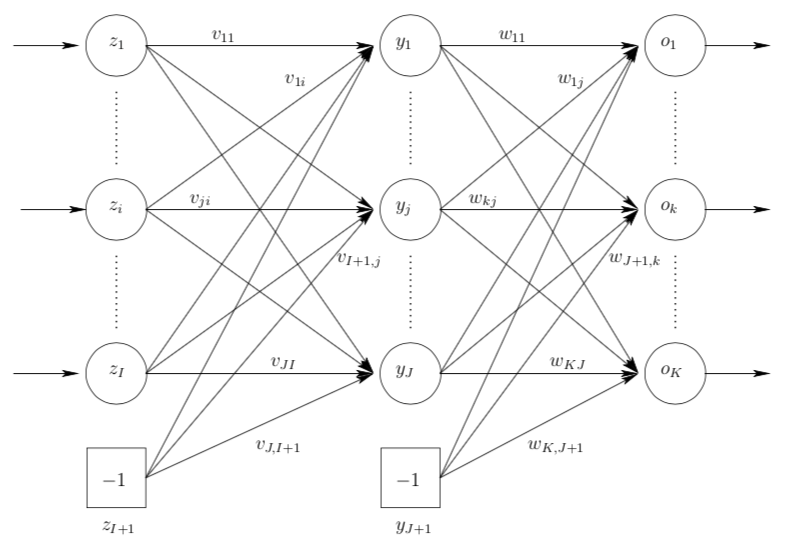
\includegraphics[width = 100mm, height = 50mm]{img/artificial_neural_network.png}
    \caption{A Multi-layer Perceptron} 
    \label{fig:ann_1}
\end{figure}

By stacking several neurons together to form an output vector $\mathbf{o} = (o_1, o_2, \cdots \o_m)$ (a layer) and then using $\mathbf{o}$ as the input to another set of neurons and so on we can form the so-called Multi-layer Perceptron (\gls{mlp}). The layers of the \gls{mlp} in between the input and output layers are called hidden layers. Figure \ graphically depicts a \gls{mlp} with one hidden layer. The process of adapting the weight matrices at each layer is called training of the Neural Network and is described in detail in \cite{Engelbrecht2007}.